\documentclass[12pt]{article}
\usepackage{fullpage}
\usepackage{enumitem}
\usepackage{amsmath}
\usepackage{amssymb}
\usepackage{amsthm}
\usepackage{array}
\usepackage{booktabs}
\usepackage{bm}
\usepackage{tikz}
\usetikzlibrary{shapes.geometric}
\usetikzlibrary{positioning}
\usetikzlibrary{decorations}
\setlength{\oddsidemargin}{-0.5cm}
\newtheorem{theorem}{Theorem}[subsection]
\newtheorem{defn}[theorem]{Definition}
\newtheorem{prop}[theorem]{Proposition}
\newtheorem{ex}[theorem]{Example}

\pgfdeclaredecoration{quasi-sirpinski}{do}{
    \state{do}[width=\pgfdecoratedinputsegmentlength, next state=do]{
        \pgfpathmoveto{\pgfpointpolar{-60}{\pgfdecoratedinputsegmentlength/2}}
        \pgfpathlineto{\pgfpointorigin}
        \pgfpathlineto{\pgfpoint{\pgfdecoratedinputsegmentlength/2}{0pt}}
        \pgfpathclose
    }
}

\begin{document}
\thispagestyle{empty}
\Large
\vspace*{2cm}
\begin{center}
\textbf{UNIVERSITY OF STRATHCLYDE}
\end{center}

\vspace*{1cm}
\begin{center}
\textbf{DEPARTMENT OF\\ MATHEMATICS AND STATISTICS}
\end{center}

\vspace*{1cm}
\begin{center}
\textbf{Inverse Semigroups}
\end{center}

\vspace*{1cm}
\begin{center}
\textbf{by}
\end{center}

\vspace*{1cm}
\begin{center}
\textbf{Adam Gaffney}\\
\end{center}

\vspace*{3cm}
\begin{center}
\textbf{MMath Mathematics}\\
\textbf{2018/19}
\end{center}

\newpage
\Large

\vspace*{1cm}
\begin{center}
\textbf{Statement of work in project}
\end{center}

\vspace*{1cm}
\begin{center}
\parbox{14cm}{
The work contained in this project is that of the author and where
material from other sources has been incorporated full acknowledgement
is made.}
\end{center}

\begin{center}
\begin{tabbing}
xxxxx\=xxxxxxxxxxxxxxx\= \kill
\\
\\
\\
\>Signed\>.........................................................\\
\\
\>Print Name\>.........................................................\\
\\
\>Date\>.........................................................\\
\end{tabbing}
\end{center}

\vspace*{5cm}
Supervised by Dr. Erzsebet Dombi 
\newpage
\normalsize
\tableofcontents
\newpage
\section{Introduction}
Semigroup theory, and subsequently inverse semigroup theory, is a broad field that is part of many different areas due to its generality. For example, it can be found in parts of computer science, more specifically the concepts of finite state automata and the study of formal languages\cite{1}. This project shall discuss the history of the field, and then we shall discuss some basic definitions of groups and semigroups to lay the foundations needed for the rest of this report. From there we will discuss the partial order, which is a concept that arises often in regards to semigroups and inverse semigroups. Then we shall discuss some well-known theorems, namely Cayley's theorem, an important theorem for groups, and the semigroup analogue in the faithful representation theorem for full transformation monoids. After this we shall discuss inverse semigroups, explore the natural partial order, which is a partial order restricted to $E(S)$ which works very nicely in inverse semigroups. Then this will lead us to discussing symmetric inverse monoids and the Wagner-Preston representation theorem which is the inverse semigroup analogue to Cayley's theorem. Throughout the project some examples will be discussed for each of these sections, as well as a couple of fleshed out examples, namely the Sierpinski triangle and the bicyclic monoid. The aim of this project will be to present these concepts so that the groundwork is there to pursue deeper research into this topic.

\section{History}
The study of semigroups, and on top of that inverse semigroups, is one that has been formally researched for at least 80 years but has actually been discussed briefly in group theory topics for 100. It has also been underlying some aspects of mathematics for much longer than that, unbeknownst to the mathematicians at the time. The first known record of the term dates all the way back to 1904, in a book by J.A. de Séguier called \textit{Élements de la Théorie des Groupes Abstraits}\cite{1}, which can be located online using the link in \cite{6}. Although it is completely written in French, it does appear that the term "semi-group" is not being used in its modern context\cite{1}, and is in fact discussing it in relation to groups, without mentioning associativity. In fact the modern usage of what makes a semigroup would not be considered until the early 1930's in which the mathematician Alfred Hoblitzelle Clifford published a paper on the theory of abstract multiplication\cite{7}. It is a passing mention in this one section in a footnote, however the actual theory is all there just ready to be built upon.\\
The 1940's, and more specifically 1940 and 1941 were really when the subject started to gain traction, due to the publishing of 3 large papers on the topic, namely \textit{Semigroups admitting relative inverses} by Clifford, \textit{Contribution \`a la théorie des demi-groupes} by a French mathematician known as Paul Dubreil, and \textit{On semi-groups} by David Rees(\cite{1},\cite{2}). These papers are still held up as the starting point for modern semigroup theory and all of the work has been building on top of the concepts introduced in these papers.\\
\\Whilst this history is applicable for the algebraic theory of semigroups, there is also the topological side of semigroups\cite{2}, although this is not discussed much in this project as we will focus more on the algebraic study. Topological semigroups have been around for much longer than the algebraic analysis, with one suggestion by J.D. Lawson even going back as far as a paper by Niels Abel from 1826\cite{8}. In this paper Abel discusses symmetric functions, and we can see that the symmetric function closely resembles that which we know about commutative semigroups, albeit not quite with the same specificity or accuracy as our modern definitions\cite{8}. However this means that we know there has likely been work done using the basic fundamentals of semigroups for almost 200 years without realising this was the case, or at least the basics of what would lead to semigroup theory were there. Of course it is not a simple one-to-one comparison as what Abel wanted to discuss was different to semigroups as far as the algebra goes, however it is interesting to note how long this field could have gone untapped.\\
\\It is argued that a Russian Mathematician Anton Kazimirovich Suschkewitsch is the first real semigroup theorist\cite{2}. He was studying generalised groups, and in his doctoral dissertation as early as 1917 he discussed the ideas of semigroups, going into more detail and discussing many of the basics of the field throughout the following 20 years.\cite{2} These would all be found later by other mathematicians, but not until many of them had reached these results independently much later.\\
\\As for inverse semigroups, they would take another 11 years before being properly introduced into the mathematical world. One of the major names in inverse semigroup theory, Victor Vladimirovich Wagner is considered to be the first to have discussed inverse semigroups, although he referred to them as \textit{generalized groups}\cite{5}. Due to the nature of the Cold War and the lack of communication between the Soviets and the Western forces, dubbed the "Iron Curtain", these ideas did not reach the West from Wagner. However a British mathematician named Gordon Preston independently introduced inverse semigroups to the Western world two years later in 1954\cite{2}. It was this lack of communication that led to the so-called "Wagner-Preston Representation Theorem" being named as such, since neither individual could really take sole credit due to the nature of the independent discoveries, and this theorem turned out to be one of the most important theorems in this field.\\

\section{Basics of Semigroup Theory}
In this section we wish to discuss some basics of both group and semigroup theory in order to showcase the parallels and differences between the fields. We will then also discuss the partial order, a concept that is very useful in both semigroups and inverse semigroups, before finally discussing two main representation theorems, namely Cayley's Theorem and the faithful representation of a semigroup $S$ with the full transformation monoid. Examples of groups and semigroups will be discussed throughout the section.
\subsection{Basic Definitions}
Here we shall discuss some of the simple definitions which form the roots of the theory, beginning with group theory and then leading into how this parallels with semigroup theory, as well as discussing idempotents and monoids.\\
\\There are many similarities between group theory and semigroup theory, so let us begin by defining what exactly makes a group.
\begin{defn}\label{defn2.1}
	Let $G$ be a non empty set, and $\cdot$ be a binary operation on $G$. Then the pairing ($G$, $\cdot$) is a \textbf{group} if
	\begin{itemize}[leftmargin=*]
		\item[] \textbf{Closed:}  For $a,b \in G$, the product $a \cdot b \in G$.
		\item[] \textbf{Associative:} For elements $a, b, c \in G, (a \cdot b) \cdot c = a \cdot (b \cdot c)$
		\item[] \textbf{Identity:}  There exists an identity element $e \in G$ such that for $a \in G, a \cdot e = e \cdot a = a.$
		\item[] \textbf{Inverse:}  Every element $a \in G$ has an inverse $a^{-1} \in G$ such that $a \cdot a^{-1} = a^{-1} \cdot a = e.$
	\end{itemize}
\end{defn}
\noindent Some examples of groups would be the real numbers $\mathbb{R}$ with addition, or the integers $\mathbb{Z}$ with addition also. We also have the concept of a subgroup.
\begin{defn}
	Let $G$ be a group, $H$ be a non empty subset of $G$, and $\cdot$ be a binary operation on $G$. Then $H$ is a subgroup of $G$ if for $g,h \in H$, $g\cdot h^{-1} \in H$.
\end{defn}
\noindent If we consider the previous examples, the integers $\mathbb{Z}$ with addition is a subgroup of the $\mathbb{R}$ with addition, as for any two elements $g,h \in \mathbb{Z}$, clearly $g+(-h) \in \mathbb{Z}$.\\
\\With these discussed, we can now proceed to define what makes a semigroup, in order to be able to work with inverse semigroups later on.
\begin{defn}\label{defnsemi}
	Let $S$ be a non-empty set, and $\cdot$ a binary operation on $S$. Then ($S$, $\cdot$) is a \textbf{semigroup} if $\cdot$ is associative. This is to say that
	\begin{center}
		$(a \cdot b) \cdot c = a \cdot (b \cdot c) \qquad $for all $a,b,c \in S$
	\end{center}
\end{defn}
\noindent Some examples of semigroups are the set of all natural numbers $\mathbb{N}$ with addition, and also with multiplication\cite{2}. Also any group is also a semigroup\cite{1}, for example the real numbers $\mathbb{R}$ under addition forms a group, and thus is also a semigroup.\\
\\For simplicity, we will represent "a semigroup ($S$, $\cdot$)" as "a semigroup $S$" from this point forward, aside from cases where the binary operation is not clear from the context. It is also standard notation to represent $a \cdot b$ as $ab$, for example associativity shall be represented as
\begin{center}
	$(ab)c=a(bc)$ \qquad for all $a, b, c \in S.$
\end{center}
This is exactly equivalent to associativity in Definition \ref{defnsemi}, however it is easier to see what is going on without the overuse of the binary operation symbol.\\
\\Just as we have the concept of subgroups in group theory, there is an equivalent concept in semigroups known as \textbf{subsemigroups}.
\begin{defn}\label{def2.10}
	A non-empty subset $T$ is a \textbf{subsemigroup} of a semigroup $S$ if for all $x, y \in T, xy \in T$. This can also be expressed as $T^2 \subseteq T$.
\end{defn}
\noindent Subsemigroups differ from subgroups in that an inverse element is not required for something to be a subsemigroup, as each element having an inverse is not required for a semigroup. A trivial example of a subsemigroup would be the semigroup $S$ itself. However another example would be the set $2\mathbb{N}^0$ of all the even non-negative integers, as this is clearly a subsemigroup of the natural numbers $\mathbb{N}^0$ with the addition operation\cite{1}.\\
Now let us define a very important concept for this field, and that is an idempotent.
\begin{defn}\label{def2.8}
	Let $S$ be a semigroup, and $e \in S$. Then $e$ is an \textbf{idempotent} if
	\begin{center}
		$e^2=ee=e$
	\end{center}
\end{defn}
\noindent In groups only one idempotent element can be found, namely the identity element, however semigroups can have multiple idempotents, and these are very useful for proving many theorems in semigroup theory, as they allow us to manipulate the elements of a semigroup in different ways. A semigroup which consists of entirely idempotents is called a \textit{band}, and the set of all idempotents of a semigroup $S$ is denoted by $E(S)$, and is clearly also a band.
This set is clearly a subset of $S$, and in fact if these idempotents commute then $E(S)$ will be a \textit{subsemigroup} of $S$. Let us prove this is the case.
\begin{ex}\label{ex2.11}
	Let $S$ be a semigroup and let $e, f \in E(S)$ and assume that $E(S)$ is commutative. Then
	\begin{center}
		$(ef)^2=efef=eeff=ef$
	\end{center}
Hence $ef \in E(S)$ and thus $E(S)$ is a subsemigroup of $S$.
\end{ex}
\noindent The definition of a semigroup lacks several key components when compared to groups, one of which is the existence of an identity element. We can see from the definition that an identity is a key requirement for a set-operator pairing to be a group, however it is not necessary for a pairing to be a semigroup. Some semigroups however, can indeed have an identity element.
\begin{defn}
	Let $S$ be a semigroup, and let $e \in S$ such that
	\begin{center}
		$es=se=s$ \qquad for all $s \in S$
	\end{center}
	Then e is an \textbf{identity} element for $S$ and the semigroup $S$ is called a \textbf{monoid}.
\end{defn}
\noindent We can show that the identity element of a monoid is unique by using contradiction. Let us assume that for a monoid $S$, we have two identity elements, $e_1, e_2 \in S$. Then we know that
\begin{center}
	$e_1=e_1e_2=e_2$
\end{center}
by the definition of the identity element, and hence the identity is always unique.\\
\\In cases where a semigroup $S$ does not contain an identity element, one can be adjoined with it to create a monoid, and this can be represented by $S \cup \{e\}$, where $e$ is the identity element being added. In this case, $S \cup \{e\}$ is known as the monoid \textit{obtained} from $S$\cite{3}. In all cases, a monoid can be denoted by $S^1$, in order to distinguish it from the base semigroup it stems from.\\
Clearly we can see that if a monoid $S^1$ exists with a binary operation $\cdot$ and identity element $e$, then if for each element $s \in S$ there exists an inverse $s^{-1} \in S$, then this monoid is a group, as it fits all the criteria for what constitutes a group.
\subsection{Partial Order}
In this section we shall discuss the partial order, it's properties and uses, as well as also discussing the concept of a lower semilattice. To begin, consider the definition of a binary relation from group theory.
\begin{defn}
	A \textbf{binary relation} $\omega$ between the sets $X$ and $Y$ is a subset of the Cartesian product $X \times Y$.
\end{defn}
\noindent In other words, an ordered pair $(x,y) \in X \times Y$ of elements $x \in X, y \in Y$ are related if $(x,y) \in \omega$, and we write this as $x \omega y$. For example, say we have the sets $X = \{1,2,3\}$ and $Y = \{3,6,9\}$. Then $\omega = \{(1,3), (2,9)\}$ would constitute a binary relation on these sets. Now we can define a partial order.
\begin{defn}\label{partial}
	Let $X$ be some set. Then a \textbf{partial order} is a binary relation $\omega \subseteq X \times X$ such that the following three properties hold;
	\begin{itemize}
		\item[] \textbf{Reflexive:} $(x,x) \in \omega$ for all $x \in X$.
		\item[] \textbf{Anti-Symmetric:} If $(x,y) \in \omega$ and $(y,x) \in \omega$ then $x$ must be equal to $y$.
		\item[] \textbf{Transitive:} If $(x,y) \in \omega$ and $(y,z) \in \omega$ then this implies that $(x,z) \in \omega$.
	\end{itemize}
\end{defn}
\noindent It is a convention when discussing partial orders to replace the binary relation $\omega$ with the symbol $\leq$, such that $(x,y) \in \omega$ is replaced by $x \leq y$. This makes partial orders much more readable, and so we shall also be using this convention for the duration of this project. 
\\For clarity, we shall also note that;
\begin{itemize}
	\item[$\bullet$] $(y,x)\in \omega$ becomes $x \geq y$
	\item[$\bullet$] $(x,y) \in \omega$ and $ x \neq y$ becomes $x < y$ and
	\item[$\bullet$] $(y,x) \in \omega$ and $x \neq y$ becomes $x>y$.
\end{itemize}
From here on we shall simply refer to the pairing $(X, \leq)$ as a partially ordered set. Now consider some non-empty subset $Y$ of the partially ordered set $(X, \leq)$. Then we can say that the element $l \in X$ is a \textit{lower bound} for $Y$ if $l \leq y$ for all $y \in Y$. This is the case for any element of $(X,\leq)$ that fits this criteria, and thus if we consider the set of all these lower bounds, it will have a maximum element we will call $m$. This maximum element is the \textit{greatest lower bound} of the subset $Y$, and it is unique and can be expressed as
	\begin{center}
		$m = \wedge \{y:y \in Y\}$.
	\end{center}
If $Y = \{a,b\}$ then we can express this as $m = a \wedge b$, and if this $m$ exists for every single $a,b \in X$ then $(X,\leq)$ is known as a \textbf{lower semilattice}. Also in a lower semilattice note that for all $a,b \in X$ we have
	\begin{center}
		$a \leq b$ if and only if $a \wedge b = a$\qquad\cite{3}.
	\end{center}
All of this together allows us to prove the following proposition, which will give us a much easier definition for lower semilattices that we can use.
\begin{prop}\label{semilattice}
	Let $(E,\leq)$ be a lower semilattice. Then we have a commutative semigroup $(E,\wedge)$ comprised of idempotents such that $a \leq b$ if and only if $a \wedge b = a$.\\
	Now consider $(E, \wedge)$ as a commutative semigroup of idempotents. Then there is a binary relation $\leq$ on E such that
	\begin{center}
		$a\leq b$ if and only if ab = a
	\end{center}
	and this forms a partial order on $E$ and following from this we get that $(E,\leq)$ is a lower semilattice.
\end{prop}
\proof
	\textbf{\underline{$\Rightarrow$:}}
	Let $(E,\leq)$ be a lower semilattice. Then clearly for $a,b,c \in E$, $(a \wedge b) \wedge c$ must be the greatest lower bound for $Y = \{(a \wedge b),c\} \subseteq E$. Likewise, $a \wedge (b \wedge c)$ must be the greatest lower bound for $Y = \{a, (b \wedge c)\}$. However since the greatest lower bound must be unique, we get
	\begin{center}
		$(a \wedge b) \wedge c = a \wedge (b \wedge c)$
	\end{center}
	And thus associativity holds, meaning that $(E, \wedge)$ is a semigroup\cite{3}. Clearly we can see that $a \wedge a = a$ for all $a \in E$ and hence $a^2 = a$, meaning all elements are idempotents. We also see that $a \wedge b$ will be equal to $b \wedge a$ for $a,b \in E$ as the greatest lower bound will not depend on order, hence $(E,\wedge)$ is a commutative semigroup.\\
	\textbf{\underline{$\Leftarrow$:}}
	Let $(E,\wedge)$ be a commutative semigroup of idempotents with $\leq$ defined as $a\leq b$ if and only if $a \wedge b = a$. We know that $a^2 = a$ and so $a\wedge a=a$ for all $a \in E$, meaning that $a \leq a$ and hence $\leq$ is reflexive.\\
	 Now assume that $a \leq b$ and $b \leq a$, then $ab = a$ and $ba = b$ and this gives us that
	\begin{center}
		$a = ab = ba = b$
	\end{center}
	since E is commutative, and hence $\leq$ is anti-symmetric.\\
	Now assume that $a \leq b$ and $b \leq c$. Then we have
	\begin{center}
		$ac = (ab)c=a(bc)=ab=a$
	\end{center}
	using the definition of the relation. Hence $a\leq c$ and $\leq$ is transitive, and thus we have shown it is a partial order.\\
	Now we wish to prove that $(E, \leq)$ is a lower semilattice. Consider the fact that $a(ab)=a^2 b =ab$. Then we have that $b(ab)=(ba)b=(ab)b=ab^2=ab$ and as such $ab \leq a$ and $ab \leq b$, thus $ab$ is a lower bound. Now consider $c \leq a$ and $c \leq b$ also, then;
	\begin{center}
		$c(ab)=(ca)b=cb=c$
	\end{center}
	and hence $c\leq ab$. This tells us that for all $a,b \in E$, $ab$ is the greatest lower bound, and so $(E,\leq)$ must be a lower semilattice.
	\qed
\\This tells us that if $(E,\leq)$ is a lower semilattice then $(E,\wedge)$ a commutative semigroup of idempotents, and the reverse is also true, making these two statements equivalent. This becomes important in demonstrating the natural partial order on semigroups in Section 4, as this makes heavy use of semilattices and so having this easier definition is beneficial.
\subsection{Faithful Representations}
In this section we wish to discuss the symmetric group, the full transformation monoid, and then leading into Cayley's Theorem and the faithful representation theorem.\\
\\This is a good point to introduce another notational convention used in semigroup theory, which is in the use of mappings. With most mappings you would represent “a mapping $\mu$ applied to an element $x$" as $\mu(x)$. However, in semigroup theory we would represent this by $(x)\mu$. Likewise, $((x)\mu)\alpha$ would be used to represent "$\mu$ applied to $x$, and then apply $\alpha$".\\
\\Let us discuss the definition of the \textit{symmetric group} $S_X$ from group theory, as this will provide a good parallel to compare to when talking about the full transformation monoid $T_X$.
\begin{defn}
	The elements of the \textbf{symmetric group} $S_X$ are permutations of a set $X$, that is all elements are bijections from the set $X$ to itself, with the group operation being the compostion of mappings.
\end{defn}
\noindent Whilst discussing the symmetric group, let us establish what the $\textbf{domain}$ and $\textbf{image}$ of the mappings in $S_X$ are. On $S_X$, we have any mapping $\alpha$ with domain $X$ and image $X$. Since all mappings are well-defined and bijections, every element in $X$ is mapped to another unique element in $X$. This holds under composition of mappings, as if you have two bijections $\alpha,\beta \in S_X$, then $\alpha$ will map an element in $X$ to another element in $X$, and $\beta$ would do the same, meaning the domain and image for $\alpha\beta$ are also both $X$.
Now let us consider the symmetric group $S_3$.
\begin{ex}
The elements of the symmetric group $S_3$ map the set $X = \{1, 2, 3\}$ onto itself using bijection mappings. Hence each element can only map to one unique element, and the range must be the full set $X$. From this, we can identify that we can only have $6$ possible permutations, and these form $S_3$
\begin{center}
	$S_3 = \{123, 132, 213, 231, 312, 321\}$, where $213$ means "$1 \mapsto 2, 2 \mapsto 1$, and $3 \mapsto 3$."
\end{center}
In fact for any $S_X$, the number of permutations will always be $n!$, where $n$ is the number of elements in $X$, as this is the maximum number of unique ways to pick $n$ numbers.\\
If we compose any two of these mappings, then we shall get another permutation from the group, and this is best displayed in the Cayley Table for $S_3$, where we can see that every composition of permutations results in another permutation in the group, as expected. Here, the mappings are composed left to right, as an example, we would take $231$ from the row, and then $132$ from the column, and this would give us $231 \cdot 132 = 321$.
	\begin{table}[htb]
	\centering
	\begin{tabular}{|r|r|r|r|r|r|r|}
		\hline
		\bm{$S_3$} & \bm{$123$} & \bm{$213$} & \bm{$132$} & \bm{$321$} & \bm{$231$} & \bm{$312$}\\
		\hline
		 \bm{$123$} & $123$ & $213$ & $132$ & $321$ & $231$ & $312$\\
		\hline
		 \bm{$213$} & $213$ & $123$ & $312$ & $231$ & $321$ & $132$\\
		\hline
		 \bm{$132$} & $132$ & $231$ & $123$ & $312$ & $213$ & $321$\\
		\hline
		 \bm{$321$} & $321$ & $312$ & $231$ & $123$ & $132$ & $213$\\
		\hline
		 \bm{$231$} & $231$ & $321$ & $321$ & $213$ & $312$ & $123$\\
		\hline
		 \bm{$312$} & $312$ & $132$ & $213$ & $132$ & $123$ & $231$\\
		\hline
	\end{tabular}
	\caption{Cayley Table for $S_3$}\label{1}
	\end{table}
\end{ex}
\noindent Now we understand the symmetric group, we can define $T_X$.
\begin{defn}
	The \textit{full transformation monoid} $T_X$ is the monoid whose elements are all maps of a set $X$ onto itself with $\cdot$, the composition of mappings operation.
\end{defn}
\noindent Just like $S_X$, the domain of $\alpha \in T_X$ is equal to $X$, since every element will be mapped to some other element, however the image is some subset of $X$, since the entire set does not need to be mapped to. The same holds for composition of mappings, the domain will again be $X$ and the image some subset $X$, namely $im(\alpha\beta)=(im(\alpha) \cap dom(\beta))\beta$.\\
It is clear to see from the definitions that $T_X$ is the semigroup analogue of $ S_X$. The main difference between them is the fact that mappings do not need to be bijections to be contained within $T_X$. This means that whilst they must be well defined, multiple elements can map to the same output element. This gives many more possibilities for mappings, as we shall see in the following example.
\begin{ex}
	Similarly to $S_3$, we can find all the elements of $T_3$ to illustrate the differences. We know that $S_X$ is contained within $T_X$, so we can start with the 6 elements of $S_3$. From there it is a case of finding the other possible mappings which account for the fact that they need not be bijections. For example, we could have the mapping $111$, that is all elements are sent to $1$. Going through all this, we end up with $27$ elements for $T_3$;
	\begin{center}
		\begingroup
			\fontsize{11pt}{12pt}\selectfont
				$\{S_3,111,112,113,121,122,131,133,211,212,221,222,223,232,233,311,313,322,323,331,332,333\}$
		\endgroup
	\end{center}
	\noindent It is worth mentioning that the number of elements found in $T_X$ will always be $n^n$, with $n$ the number of elements in $X$. This is the number of mappings possible including any repeated elements, and this tells us that the size of $T_X$ grows exponentially as the size of $X$ increases.\\
\\The Cayley table for this would be too large to display here, however the same applies as with $S_3$, in that if you take any two of these mappings and compose them, you will get another mapping also contained in $T_X$. For example, take $112 \cdot 213$. Then $1 \mapsto 1$ from $112$, then to $2$ from $213$. Likewise, $2 \mapsto 1 \mapsto 2$, and $3 \mapsto 2 \mapsto 1$. This means that composing $122$ with $213$ is the same as the mapping $221$, which is clearly also a member of $T_X$. This can be done for any combination of elements of $T_X$.
\end{ex}
\noindent Another point of note is that $S_X$ is in fact a subgroup of $T_X$. As all elements of $S_X$ are bijections, they will be contained within $T_X$ as this contains all maps, including all bijections, hence $S_X$ is a subset of $T_X$. Now we simply apply the subgroup test to show this is true.\\
Let $a, b \in S_X$, then there exists an inverse $b^{-1} \in S_X$. As $S_X$ is a group, we know that the binary operation with any two elements of the group is also a member of the group, hence $ab^{-1} \in S_X$ and thus $S_X$ is a subgroup of $T_X$.\\
\\Now we can begin to discuss the concept of a \textit{morphism} (also known as a \textit{homomorphism}).
\begin{defn}
	A mapping $\mu:S\to T$, where $S$ and $T$ are semigroups is called a \textbf{morphism} if, for all $x, y \in S$
	\begin{center}
		$(xy)\mu = (x\mu)(y\mu)$
	\end{center}
	If $S$ and $T$ are monoids, then for $\mu$ to be a morphism the extra condition must hold that
	\begin{center}
		$e_S\mu=e_T$
	\end{center}
	Where $e_S$ and $e_T$ are the identity elements of $S$ and $T$ respectively.
\end{defn}
\noindent There are several extra subcatagories of morphisms also.
\begin{defn}\label{def2.13}
	Let a mapping $\mu:S\to T$ be a morphism for semigroups $S$ and $T$. Then we have;
	\indent
	\begin{itemize}
		\item[a)] $\mu$ is a \textbf{monomorphism} if it is injective, that is if for $x, y \in S, x\mu = y\mu$ implies that $x = y$.
		\item[b)] $\mu$ is an \textbf{endomorphism} if it maps from $S$ into itself.
		\item[c)] $\mu$ is an \textbf{automorphism} if it is an endomorphism and also a bijection.
		\item[d)] $\mu$ is an \textbf{isomorphism} if it is invertible, in other words $\mu\mu^{-1} = I_S$ and $\mu^{-1}\mu = I_T$ where $I_S$ and $I_T$ are the identity maps of $S$ and $T$ respectively.
	\end{itemize}
\end{defn}
\noindent If we focus on Definition \ref{def2.13} d) for now, we can show a small but useful result quite easily.
\begin{prop}\label{prop2.14}
	Let $S$ and $T$ be semigroups and let $\mu:S\to T$ be a morphism. Then 
	\begin{center}
		$\mu$ is an isomorphism $\iff$ $\mu$ is a bijection.
	\end{center}
\end{prop}
\proof
	\textbf{\underline{$\Leftarrow$:}}
		Let us initially assume that $\mu$ is a bijection, then for each element $t \in T$, there exists a unique element $s \in S$ such that $(s)\mu = t$. Clearly from this there must also be a map $\mu^{-1}:T \to S$ such that $s = (t)\mu^{-1}$, and $\mu\mu^{-1} = I_S, \mu^{-1}\mu = I_T$. Hence $\mu$ is an isomorphism.\\
	\\\textbf{\underline{$\Rightarrow$:}}
		Now let us assume that $\mu$ is an isomorphism. Assume that $(x)\mu = (z)\mu$ for $x, z \in S$. Then there exists $\mu^{-1}:T\to S$ such that
		\begin{center}
			$(x)(\mu\mu^{-1}) = ((x)\mu)\mu^{-1} = ((z)\mu)\mu^{-1} = (z)(\mu\mu^{-1})$
		\end{center}
		and since $\mu$ is an isomorphism, this gives $xI_S = zI_S$, which implies that $x = z$, hence $\mu$ is injective.
		Let $y \in T$ and $\mu^{-1}:T\to S$. Assume that $y\mu^{-1} = x$, then it follows that
		\begin{center}
			$y\mu^{-1}\mu = y = x\mu$	for $x \in S$.
		\end{center}
		Thus $\mu$ is surjective as for all $y \in T$, as there exists an $x \in S$ such that $\mu x = y$. This implies that $\mu$ is bijective and the proposition holds.
	\qed\\
\\Often showing one side of Proposition \ref{prop2.14} is easier than the other when working with a mapping, and so thanks to this we need only show that side is true, and the other will follow from that.\\
\\Now let us define what a \textit{faithful representation} is, as it will be necessary for the upcoming theorems.
\begin{defn}
	A morphism $\mu:S \to T_X$ is a representation of $S$, and it is called a \textbf{faithful representation} if this $\mu$ is injective.
\end{defn}
\noindent With these concepts established, we can now discuss a couple of very important theorems in group and semigroup theory: Cayley’s Theorem and an analogous theorem for semigroups using the full transformation monoid.
\begin{theorem}[\textbf{Cayley's Theorem}]
	Let $G$ be a group. Then $G$ is isomorphic to a subgroup of the symmetry group $S_G$.
\end{theorem}
\proof
	Define the mappings
		\begin{alignat*}{2}
			L_g:G \to G & \qquad	\text{and}\qquad 	\mu:G\to S_G.\\		
			x\mapsto gx & \qquad \qquad \qquad \quad g\mapsto L_g
		\end{alignat*}
	First we want to show that $L_g$ is indeed an element of the symmetric group, which means it is bijective. Assume that for some $x,y,g \in G, (x)L_g=(y)L_g$. Then $gx = gy$ and multiplying by $g^{-1}$ on the left gives us $x=y$, which shows injectivity.\\
	Now consider $y \in G$, then we know that $g^{-1}y \in G$. Then we have that $(g^{-1}y)L_g = gg^{-1}y = y$. This implies that $L_g$ is surjective and as such is bijective, hence $L_g \in S_G$. \\
	We now want to show that $\mu$ is an injective homomorphism. Consider $g,h,j \in G$, then we have
	\begin{center}
		$(j)L_{gh}=(gh)j=g(hj)=(hj)L_g=(j)L_hL_g$
	\end{center}
	This implies that $(gh)\mu = (h)\mu(g)\mu$ and hence $\mu$ is a homomorphism.\\
	Now consider $g,h,z \in G$ such that $(g)\mu = (h)\mu$. Then we get $(z)L_g = (z)L_h$, which implies that $gz=hz$. As $G$ is a group, there must exist $z^{-1}$ such that $zz^{-1} = id$, hence multiplying on the right by $z^{-1}$ on both sides gives $g=h$, which implies that $\mu$ is injective and so $G$ is isomorphic to a subgroup of $S_G$.
	\qed\\
\\This is incredibly powerful, as it means that by studying subgroups of the symmetric group, one can easily generalise any results to every group, and so having an analogue to this like we do in this next theorem is incredibly useful for semigroups too. 
\begin{theorem}
	If $S$ is a semigroup and $X=S^1$ then there is a \textbf{faithful representation} $\mu:S\to T_S$.
\end{theorem}
\proof
	For $a \in S$, let us define the mappings
		\begin{alignat*}{2}
			\rho_a:S^1 &\to S^1  \qquad	\text{and}\qquad 	\mu:S&\to T_S.\\		
			x&\mapsto ax  \qquad \qquad \qquad \quad s&\mapsto \rho_a
		\end{alignat*}
	Just like with Cayley's Theorem, we wish to show that $\mu$ is an injective morphism. Let $a,b \in S$ such that $a\mu=b\mu$. This implies that $\rho_a=\rho_b$, which implies that $ax=bx$ for all $x \in S^1$, which includes the identity $1_s$, hence $a1=b1$ which implies that $a=b$, and so $\mu$ in injective.
	Let $a,b \in S^1$. Then
	\begin{center}
		$x(\rho_a\rho_b)=(x\rho_a)\rho_b=(ax)\rho_b=b(ax)=(ba)x=x\rho_{ab}$
	\end{center}
	This shows that $(a)\mu(b)\mu=(ab)\mu$ and hence $\mu$ is a morphism.
	\qed\\
\\This theorem works similarly to Cayley’s Theorem in that it allows us to carry out work on the full transformation monoid and any subgroup of it, and then any results that work on this can operate on any monoid.
\section{Inverse Semigroup Theory}
In this section we shall introduce the concept of regular semigroups and this will lead us in nicely to inverse semigroups. We shall discuss some properties of inverse semigroups as well as inverse semigroup morphisms, and then finally we shall discuss the natural partial order, and just like the previous section examples shall be included throughout the section.
\subsection{Basics of Inverse Semigroups}
Let us begin by defining a regular semigroup, something that is important for inverse semigroups.
\begin{defn}
	Let $S$ be a semigroup. Then we would call this semigroup \textbf{regular} if for each $s \in S$, we have an $x \in S$ such that $s=sxs$.
\end{defn}
\noindent One example of a regular semigroup is in fact the full transformation monoid $T_X$\cite{1}.
\begin{ex}\label{ex2.18}
	Take the elements $133,132 \in T_3$. Then we can see that $133 \cdot 132 \cdot 133 = 133$ under the composition of mappings, and this can apply to any element of the monoid. In fact in this case, using $112, 122$ and $132$ as our "$x$" will all give the desired result.
\end{ex}
\noindent We can also see an example of a semigroup that is not regular, in this case $(\mathbb{N}, +)$.
\begin{ex}
	Take the semigroup $(\mathbb{N},+)$. This is clearly not regular, as $\mathbb{N}$ consists entirely of positive numbers, and so it is not possible for $s = sxs$ for any $s,x \in (\mathbb{N},+)$, as this would require a negative or zero.
\end{ex}
\noindent With the definition of a regular semigroup this is a good time to move onto what we call inverse semigroups, and it will become apparent how regular semigroups are linked to these inverse semigroups.\\
\\The best place to begin here would be by first defining what exactly an inverse is. In group theory, an inverse of an element $g$ of a group $G$ would be represented by $g^{-1}$ and is also a member of $G$, with the property that $gg^{-1} = e_G$ where $e_G$ is the identity element of $G$. However, when working in semigroups we are of course not able to guarantee that a semigroup $S$ will contain an identity element, and so we need to give a much broader definition of what an inverse is.
\begin{defn}
	Let $S$ be a semigroup and let $s \in S$. Then an element $s^\prime \in S$ is called the \textbf{inverse} of $s$ if
	\begin{center}
		$ss^\prime s = s$	and	$s^\prime ss^\prime= s^\prime$
	\end{center}
\end{defn}
\noindent This definition clearly applies for all groups where $ss^\prime=s^\prime s=id$, but adds an extra layer so that inverses in semigroups, where an identity is not a necessity, can be considered. Another thing that can immediately be spotted is that this definition is very similar to the definition for a regular semigroup, and while this is relevant we must be careful when looking at this. Let us use Example \ref{ex2.18} to demonstrate why.
\begin{ex}\label{ex3.2}
	Take $112,122,132,133 \in T_3$. We know that $T_3$ is regular and with these cases, $133=133\cdot132\cdot133$. This gives us the first step for $133$ and $132$ to be inverses, so now let us find the result of $132\cdot133\cdot132$ under composition of mappings. We get that $1 \mapsto 1, 2 \mapsto 2$ and $3 \mapsto 2$.\\
	However, this tells us that $132\cdot133\cdot132=122$, hence $133$ and $132$ are not inverses. Thus you cannot assume that elements $s,x \in S$ which follow regularity are necessarily inverse to one another.\\
	If we do this with $112$ and $122$ however, we find that these are both inverses to $133$, so when looking for inverses a good place to start is checking elements that satisfy $s=sxs$.
\end{ex}
Example \ref{ex3.2} demonstrates well that the inverse in semigroups is not related to the identity, as the identity mapping for $T_3$ is $123$, which is not obtained from any combination of $133$ with the inverses $112$ and $122$.\\
\begin{defn}\label{def3.3}
	A semigroup $S$ is called an \textbf{inverse semigroup} if each element $s \in S$ has a \textbf{unique} inverse $s^{-1}$.
\end{defn}
\noindent We can immediately draw some conclusions from the fact that the inverse must be unique, for example the full transformation monoid $T_X$ cannot be an inverse semigroup, as we saw in Example \ref{ex3.2} that the element $133$ has at least two inverses, namely $112$ and $122$. Also it is clear to see that every inverse semigroup must be regular but the converse is not true. Let us show this with our next proposition.
\begin{prop}
	Every inverse semigroup $S$ is regular, but not every regular semigroup is an inverse semigroup.
\end{prop}
\proof
	Let $S$ be an inverse semigroup. Then for $s \in S$ there exists an inverse $s^{-1} \in S$ such that
	\begin{center}
		$s=ss^{-1}s \qquad and \qquad s^{-1}=s^{-1}ss^{-1}$.
	\end{center}
	It follows directly from this definition that $S$ is regular, as we can take $s^{-1} = x$, giving $s=sxs$ for some $s,x \in S$, and so every inverse semigroup is regular.\\
	\\For the second part of the proposition, we simply use Example \ref{ex3.2}, as this clearly shows that $T_X$ is not an inverse semigroup, as the element $133$ has multiple inverses.
	\qed\\
\\We can now bring back idempotents from Definition \ref{def2.8} and prove an important proposition that will help us with future proofs.
\begin{prop}\label{prop3.4}
	A regular semigroup $S$ is an inverse semigroup if and only if its idempotents commute.
\end{prop}
\proof
	\textbf{\underline{$\Rightarrow$:}}
		Let $S$ be an inverse semigroup and let $e,f \in S$ be idempotents. Initially let us show that $ef$ has an inverse that is idempotent as this will be useful for the proof. So let $x=(ef)^{-1}$ be any inverse of our product of idempotents $ef$ such that $(ef)(ef)^{-1}(ef)=(ef)$ and $(ef)^{-1}(ef)(ef)^{-1}=(ef)^{-1}$. Then we have
		\begin{center}
			$(ef)=efxef=effxeef=(ef)fxe(ef)$\\[5mm]
			$fxe=f(xefx)e=fxefxe=fx(ee)(ff)xe=(fxe)ef(fxe)$.\\
		\end{center}
		We can see that $ef$ and $fxe$ are inverses, and that $fxe$ = $fxefxe$, hence $fxe$ is an idempotent inverse of $ef$.\\
		Now since $S$ is an inverse semigroup, we know that each inverse is unique, and this implies that $x=fxe$ and hence $x$ is also idempotent. Also any idempotent is its own inverse, as 
		\begin{center}
			$eee=ee=e$
		\end{center}
		and since $x$ is the inverse of $ef$ this means that $x = ef$ and thus $ef$ is idempotent itself. As both $e$ and $f$ are idempotents, this means that $E(S)$ is closed under multiplication, and as such $fe$ must also be idempotent. Now we can see that $fe$ and $ef$ are inverses, as
		\begin{center}
			$(ef)fe(ef)=efef=ef$	and	$(fe)ef(fe)=fefe=fe$
		\end{center}
		so both $fe$ and $ef$ are inverses for $ef$, meaning that $fe=ef$, and hence the idempotents commute.\\
	\\\textbf{\underline{$\Leftarrow$:}}
		Let $S$ be a regular semigroup with commutating idempotents, and let $u,v \in S$ be two inverses of $x \in S$ such that $u = uxu, x=xux$ and $v=vxv, x=xvx$. Then we can say that
		\begin{center}
			$u=uxu=uxvxu=(ux)(vx)u$
		\end{center}
		As idempotents commute, and $ux$ and $vx$ are idempotents since $(ux)(ux)=(uxu)x=ux$ and $(vx)(vx)=(vxv)x=vx$, we get
		\begin{center}
			$(ux)(vx)u=(vx)(ux)u=vx(uxu)=vxu=v(xvx)u=v(xv)(xu)$
		\end{center}
		Again by commuting idempotents $vx$ and $xv$ we get
		\begin{center}
			$v(xv)(xu)=v(xu)(xv)=v(xux)v=vxv=v$
		\end{center}
		And thus we have that $u=v$, meaning that the inverse is unique and $S$ is an inverse semigroup.
	\qed\\
\\Proposition \ref{prop3.4} is very powerful for proofs under inverse semigroups, as it allows us to manipulate elements in order to complete some later proofs, as we shall see in the upcoming Theorem \ref{thm3.7}. Commutativity is a luxury that is not often found in the study of groups, semigroups and such, due to the generality of the topic meaning it cannot be assumed. So being able to use commutativity is always a fantastic tool in the toolbox.\\
\\There are a few properties from group inverses that carry over to generalised inverses for inverse semigroups. 
\begin{prop}\label{inverseprop}
Let $S$ be an inverse semigroup. Then we have;
	\begin{itemize}
		\item[\textbf{(a)}] $(s^{-1})^{-1} = s$ for $s \in S$
		\item[\textbf{(b)}] For $s \in S$ with the inverse element $s^{-1} \in S$, $ss^{-1}$ and $s^{-1}s$ are idempotent.
		\item[\textbf{(c)}] $(st)^{-1} = t^{-1}s^{-1}$ for $s,t \in S$
		\item[\textbf{(d)}] If $e \in S$ is an idempotent, then $ses^{-1}$ is also an idempotent.
	\end{itemize}
\end{prop}
\proof
	\textbf{(a)} Clearly this is the case, as for an element $s \in S$ where $S$ is an inverse semigroup, $s=ss^{-1}s$ and $s^{-1}=s^{-1}ss^{-1}$. Hence $s$ is the inverse of $s^{-1}$, and so $s = (s^{-1})^{-1}$.\\
	\textbf{(b)} Consider $ss^{-1}$, then we can see that
	\begin{center}
		$(ss^{-1})(ss^{-1})=(ss^{-1}s)s^{-1}=ss^{-1}$.
	\end{center}
	Likewise, for $s^{-1}s$ we have
	\begin{center}
		$(s^{-1}s)(s^{-1}s)=(s^{-1}ss^{-1})s=s^{-1}s$.
	\end{center}
	Hence this property holds.\\
	\textbf{(c)} Consider $st$. Then we have
	\begin{center}
		$st = s(s^{-1}s)(tt^{-1})t=s(tt^{-1})(s^{-1}s)t=(st)(t^{-1}s^{-1})(st)$.
	\end{center}
	Now consider $t^{-1}s^{-1}$, then we have
	\begin{center}
		$t^{-1}s^{-1}=t^{-1}(tt^{-1})(s^{-1}s)s^{-1}=t^{-1}(s^{-1}s)(tt^{-1})s^{-1}=(t^{-1}s^{-1})st(t^{-1}s^{-1})$.
	\end{center}
	Hence $(st)^{-1} = t^{-1}s^{-1}$.\\
	\textbf{(d)} Consider $ses^{-1}$. Then we have
	\begin{center}
		$(ses^{-1})(ses^{-1})=s(e(s^{-1}s))es^{-1}=(ss^{-1}s)ees^{-1}=se^2s^{-1}=ses^{-1}$.
	\end{center}
	\qed\\
We can also see that $s^{-1}es$ is idempotent, and this can be proven in a similar manner to the proof of part \textbf{(d)}.\\
The fact that the generalized inverse behaves similarly to the group inverse is rather nice, as we can treat it in a similar way and use these properties in future proofs.\\
\\Consider the full transformation monoid $T_3$. From Example \ref{ex2.18}, we know that $T_3$ is a regular semigroup, and from Example \ref{ex3.2} and Definition \ref{def3.3} we know that it is \textit{not} an inverse semigroup. Therefore Proposition \ref{prop3.4} tells us that the idempotents in $T_3$ do not commute, and we can show this to make it clear this holds true.
\begin{ex}
	To show that $T_3$ does not have commutating idempotents, we only need to show that there is a single counter-example, so consider the mappings $111,222 \in T_3$. Clearly these are idempotents, as $111 \cdot 111 = 111$ and $222 \cdot 222 = 222$. However
	\begin{center}
		$111 \cdot 222 = 111$ \quad	and \quad	$222 \cdot 111 = 222$.
	\end{center}
	These are not equal and as such do not commute, so it holds that $T_3$ is not an inverse semigroup.
\end{ex}
\noindent In the last section, we considered group homomorphisms and semigroup homomorphisms, so now is a good time to tackle \textit{inverse semigroup morphisms}.
\begin{defn}
	A semigroup morphism $\mu:S\to T$ is an \textbf{inverse semigroup morphism} if for any $s \in S$
	\begin{center}
		$s^{-1}\mu=(s\mu)^{-1}$ holds.
	\end{center}
\end{defn}
\noindent We can then use this to prove the following theorem.
\begin{theorem}\label{thm3.7}
	Let $S$ be an inverse semigroup, $T$ a semigroup and let $\mu:S \to T$ be a surjective semigroup morphism. Then 
	\begin{itemize}
			\item[\textbf{(a)}]$T$ is an inverse semigroup and 
			\item[\textbf{(b)}]$\mu$ is an inverse semigroup morphism.
	\end{itemize}
\end{theorem}
\proof
	\textbf{(a)} For every $t \in T$, we can express it as $s\mu$ for $s \in S$. For $s^{-1} \in S$, we have
	\begin{center}
		$(s\mu)(s^{-1}\mu)(s\mu)=(ss^{-1}s)\mu=s\mu$ \quad and\\
		$(s^{-1}\mu)(s\mu)(s^{-1}\mu)=(s^{-1}ss^{-1})\mu=s^{-1}\mu$
	\end{center}
	and so $s^{-1}\mu$ is an inverse for $s\mu$ in $T$. This tells us that $T$ is regular, as this applies for all $t \in T$.\\
	Now consider idempotents $e,f \in S$. Then it follows that $e\mu=g$ and $f\mu=h$ for some $g,h \in T$. Also $e\mu$ is idempotent, as
	\begin{center}
		$e\mu e\mu = (ee)\mu=e\mu$
	\end{center}
	hence $g$ and $h$ must both be idempotent. Using all this we get
	\begin{center}
		$gh=e\mu f\mu=(ef)\mu=(fe)\mu=f\mu e\mu=hg$
	\end{center}
	Thus showing that $T$ is a regular semigroup with commuting idempotents, and by Proposition \ref{prop3.4} we have that $T$ is an inverse semigroup. \\
	\\\textbf{(b)} This easily follows from the beginning of (a), as for every $s \in S, s^{-1}\mu$ is an inverse for $s\mu$, and since $T$ is an inverse semigroup this inverse is unique, that is;
	\begin{center}
		$s^{-1}\mu = (s\mu)^{-1}$
	\end{center}
	and so $\mu$ is in fact an inverse semigroup morphism.
	\qed\\
This proof used a nice combination of Theorem 5.1.4 from Howie's Book \cite{3} and also Lemma 2.7 from Mark Lawson's notes \cite{4}, both of which are concise proofs I have expanded upon here. Before moving onto our next section now would be a good time to discuss the \textbf{natural partial order}.\\
\subsection{Natural Partial Order}
In this section we shall discuss the natural partial order, its relation to the partial order and some properties it holds.\\
\\The natural partial order, as the name implies, is a type of partial order which is defined for inverse semigroups in a much more natural way than the regular partial order discussed in Section 2.
\begin{defn}
	The \textbf{natural partial order} is defined on an inverse semigroup $S$ such that for $a,b \in S$, $a \leq b$ if there is an idempotent $e$ in $S$ such that $a=eb$.
\end{defn}
\noindent Of course it is in the name that this is a \textit{partial order}, however lets go ahead and prove this using Definition \ref{partial} so it is clear.
\begin{prop}
	The natural partial order is a partial order. In other words, it is reflexive, anti-symmetric and transitive.
\end{prop}
\proof
	For this to be a partial order, we wish to prove that it is reflexive, anti-symmetric and transitive, so let us first show it is reflexive.\\
	To show it is reflexive, we want to show that there is some idempotent $e \in S$ such that $a=ea$. Clearly we can see that as $S$ is an inverse semigroup and the product of an element with its inverse is idempotent by Proposition \ref{inverseprop}, $a =(aa^{-1})a$ works, and so $a \leq a$.\\
	To show it is anti-symmetric we want to show that given $a \leq b$ and $b \leq a$, this implies that $a=b$. If $ a\leq b$ and $b\leq a$ then $a=eb$ and $b=fa$ respectively, where $e$ and $f$ are idempotents in $S$. Thus we have
	\begin{center}
		$a=eb=efa=fea=fe(eb)=feb=fa=b$
	\end{center}
	and hence $\leq$ is anti-symmetric.\\
	To show it is transitive, we want to show that given $a \leq b$ and $b \leq c$, this implies that $a \leq c$. As $a \leq b$ and $b \leq c$, we have that for idempotents $e,f \in S$, $a=eb$ and $b=fc$. It follows from this that $a =e(fc)=(ef)c$ where $ef$ is also idempotent since $E(S)$ is closed under the binary operation. Therefore we have $a \leq c$ and hence the natural partial order is indeed a partial order.
	\qed\\
There are a few nice properties that the natural partial order has that makes it nice to work with as we shall demonstrate with the following proposition.
\begin{prop}\label{natprop}
	Let $S$ be an inverse semigroup and let $\leq$ be the natural partial order. Then the following properties hold;
	\begin{itemize}
		\item[\textbf{(a)}] If $a \leq b$ and $c \in S$ then it follows that $ac \leq bc$ and $ca \leq cb$.
		\item[\textbf{(b)}] If $a \leq b$ then $a^{-1} \leq b^{-1}$.
		\item[\textbf{(c)}] For idempotents $e$ and $f$, $e \leq f$ if and only if $e = ef = fe$.
	\end{itemize}
\end{prop}
\proof
	\textbf{(a)} By definition of the natural partial order $a=eb$ for some idempotent $e \in S$. Hence
		\begin{center}
			$ac = (eb)c=e(bc)$
		\end{center}
		and so $ac \leq bc$. For the second part, we have
		\begin{center}
			$ca=c(eb)=cc^{-1}c(eb)=c((c^{-1}c)e)b$.
		\end{center}
		We know idempotents commute in an inverse semigroup by Proposition \ref{prop3.4}, and from Proposition \ref{inverseprop} \textbf{(b)} we know any element multiplied with its inverse is idempotent, and so we have
		\begin{center}
			$c((c^{-1}c)e)b = c(e(c^{-1}c))b=(cec^{-1})cb$
		\end{center}
		From Proposition \ref{inverseprop} \textbf{(d)}, we have that $cec^{-1}$ is idempotent and therefore $ca \leq cb$.\\
	\textbf{(b)} Consider $a^{-1}$. Then we have 
	\begin{center}
		$a^{-1}=(eb)^{-1}=b^{-1}e^{-1}$.
	\end{center}
	As established in the proof of Proposition \ref{prop3.4}, any idempotent is its own inverse, and so we have
	\begin{center}
		$b^{-1}e^{-1}=b^{-1}e=b^{-1}(bb^{-1})e=(b^{-1}eb)b^{-1}$
	\end{center}
	and from Proposition \ref{inverseprop}, we have that $b^{-1}eb$ is idempotent, and so $a^{-1} \leq b^{-1}$.\\
	\textbf{(c)} This is a trivial property to prove, as clearly if $e \leq f$, then by definition $e = ef$, and since idempotents commute $ef=fe$. Also for the reverse, if $e=ef=fe$, then by definition it follows that $e \leq f$.
	\qed\\
The natural partial order is rather useful in inverse semigroups which is owed in part to the fact it introduced an idempotent into the equation. Idempotents in inverse semigroups have many useful properties as demonstrated here, as it introduced commutativity, giving us much more flexibility for algebraic manipulation.\\ 
\\The natural partial order is well suited to the subject of our next section, the \textbf{symmetric inverse monoid}.
\section{The Wagner-Preston Representation Theorem}
In this section we shall discuss the symmetric inverse monoid, what it constitutes and this will all tie into proving the Wagner-Preston representation theorem, an important theorem in the study of inverse semigroups. From this we shall then discuss some examples of the applications of inverse semigroups, so as to better illustrate the uses of this.
\subsection{Symmetric Inverse Monoid}
In this section we wish to define the symmetric inverse monoid, discuss some properties of this, and then use this to define and discuss the Wagner-Preston representation theorem.\\
\\Starting off this section let us define what exactly the symmetric inverse monoid is.
\begin{defn}
	The \textbf{symmetric inverse monoid $I_X$} is the set of all partial bijections from one subset of the set $X$ to another, with the composition of mappings operation.
\end{defn}
\noindent Up until now we have been working with mappings that map the entire set to some image. However partial mappings are those that do not map the entire set, that is the domain of a partial mapping $\mu$ is a subset of $X$, or $dom(\mu) \subseteq X$. The following is a small example found in Howie's book which demonstates this well\cite{3}.
\begin{ex}\label{ex4.2}
	Let $X$ be a non-empty set defined by $X = \{1,2,3\}$. Then the symmetric inverse monoid $I_X$ will be $I_3$, with the all the element of $S_3$ , the empty mapping and the following partial bijections;
	\begin{center}
		$\left(
		\begin{array}{c}
		1  \\
		1 
		\end{array}
		\right)$,
		$\left(
		\begin{array}{c}
		1  \\
		2 
		\end{array}
		\right)$,
		$\left(
		\begin{array}{c}
		1  \\
		3 
		\end{array}
		\right)$
	\end{center}
	The bijections for the domain=$\{2\}$ and domain=$\{3\}$ follow similarly to above, giving $9$ total with a domain of size $1$. We also have
	\begin{center}
		$\left(
		\begin{array}{c c}
		1  & 2\\
		1  & 2
		\end{array}
		\right)$,
		$\left(
		\begin{array}{c c}
		1  & 2\\
		2  & 1
		\end{array}
		\right)$,
		$\left(
		\begin{array}{c c}
		1  & 2\\
		1  & 3
		\end{array}
		\right)$,
		$\left(
		\begin{array}{c c}
		1  & 2\\
		3  & 1
		\end{array}
		\right)$,
		$\left(
		\begin{array}{c c}
		1  & 2\\
		2  & 3
		\end{array}
		\right)$,
		$\left(
		\begin{array}{c c}
		1  & 2\\
		3  & 2
		\end{array}
		\right)$
	\end{center}
	The bijections for domain = $\{1,3\}$ and domain = $\{2,3\}$ follow similarly to above, which gives us $18$ total with a domain of size $2$, and hence in total $I_3$ consists of $34$ elements. 
\end{ex}
\noindent In this example we can see that partial mappings provide much more flexibility with mapping elements of a set as the entire set does not need to be used, and these can be used to describe partial symmetries such as comparing edges of the equilateral triangle, or many different symmetries in the \textit{Sierpinski Triangle} which shall be covered later. \\
\\For $S_X$ and $T_X$ we established the domain and image of their mappings under composition of mappings so let us now consider, what are the domain and image for composition of mappings on $I_X$? The answer is actually slightly more difficult than for that of $S_X$ and $T_X$ due to the existence of partial mappings, meaning that not every element in the set X is contained in the domain of $\alpha \beta \in X$. The image of $\alpha \beta \in I_X$ consists of the elements in the image of $\beta$ that lie exclusively in the intersection of $im(\alpha)$ and $dom(\beta)$, in other words our image is $im(\alpha\beta)=(im(\alpha) \cap dom(\beta))\beta$.\\
Also, we know that we need those elements in the domain of $\alpha$ which map to the intersection of $im(\alpha)$ and $dom(\beta)$, so if we take the \textbf{inverse} of $\alpha$ and map this intersection back to $dom(\alpha)$, then we will get the elements in the domain which map to the intersection, and in turn map to the image of $\alpha\beta$. Hence we have $dom(\alpha\beta)=(im(\alpha) \cap dom(\beta))\alpha^{-1}$.\\
\\The image below is an excellent representation of how composition of mappings works with $I_X$, and whilst it was based off of the image in Howie's book, is a pretty standard representation found in many inverse semigroup resources. This gives a much clearer picture of how composition of mappings is actually working in the symmetric inverse monoid.
\begin{center}
	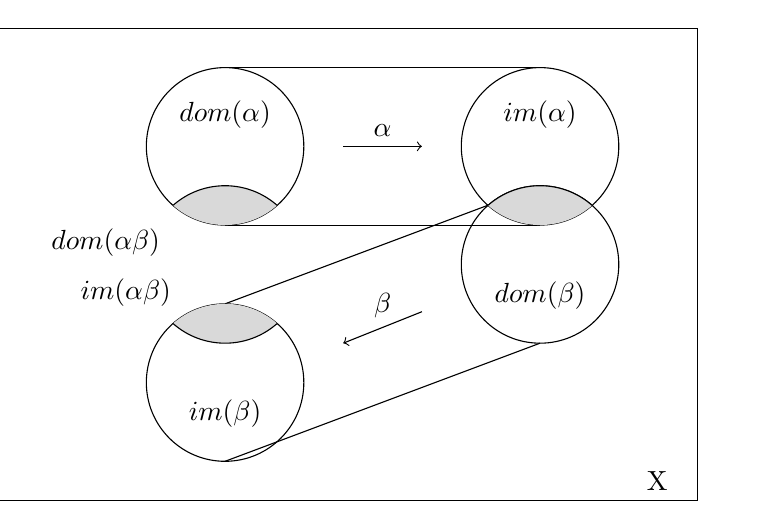
\begin{tikzpicture}
		\draw (9,0) -- (0,0);
		\draw (9,0) -- (9,-6);
		\draw (0,-6) -- ++(8,0) -- ++(0.98,0) node[midway,above] {X} -- ++(0.02,0);
		\draw (0,0)--(0,-6);
		\draw (3,-1.5) circle(1); %dom(\alpha)%
		\draw (7,-1.5) circle(1); %im(\alpha)%
		\draw (3,-4.5) circle(1); %im(\beta)%
		\draw (7,-3) circle(1); %dom(\beta)%
		\draw (7,-2) -- (3,-3.5);
		\draw (7,-4) -- (3,-5.5);
		\draw (7,-0.5) -- (3,-0.5);
		\draw (7,-2.5) -- (3,-2.5);
		\draw[->] (4.5,-1.5) -- ++(0.5,0) node[above] {$\alpha$} -- ++(0.5,0);
		\draw[<-] (4.5,-4) -- ++(0.5,0.2) node[above] {$\beta$} -- ++(0.5,0.2);
		\begin{scope}
			\clip (3,-1.5) circle(1);
			\draw[fill=gray!30] (3,-3) circle(1);
		\end{scope}
		\begin{scope}
			\clip (3,-4.5) circle(1);
			\draw[fill=gray!30] (3,-3) circle(1);
		\end{scope}
		\begin{scope}
			\clip (7,-1.5) circle(1);
			\draw[fill=gray!30] (7,-3) circle(1);
		\end{scope}
		\node[below =0.5mm of {122:-2.8)}]{$dom(\alpha \beta)$};
		\node[below left=1mm of {(130:-3.9)}]{$im(\alpha \beta)$};
		\node[above=1mm of {(3,-1.5)}]{$dom(\alpha)$};
		\node[above=1mm of {(7,-1.5)}]{$im(\alpha)$};
		\node[below=1mm of {(7,-3)}]{$dom(\beta)$};
		\node[below=1mm of {(3,-4.5)}]{$im(\beta)$};
	\end{tikzpicture}
\end{center}
Before we can continue however, note that currently, $I_X$ is an inverse monoid on name alone, so let us show this is the case.
\begin{prop}
	The symmetric inverse monoid $I_X$ is an inverse monoid.
\end{prop}
\proof
	Since $I_X$ consists of partial bijections, this means that any $\alpha \in I_X$ is a partial bijection. We can say that there exists an inverse $\alpha^\prime \in I_X$ such that
	\begin{center}
		$dom(\alpha^\prime) = im({\alpha}) \quad$ and \quad $im(\alpha^\prime)=dom({\alpha})$.
	\end{center}
	From the definition of the inverse this tells us that $\alpha\alpha^\prime\alpha=\alpha$ and $\alpha^\prime\alpha\alpha^\prime = \alpha^\prime$ and since $\alpha$ can be any mapping in $I_X$, every element in $I_X$ is regular, and so it follows that $I_X$ is regular.
	\\Now consider $\alpha$ to be an idempotent, with $\alpha^\prime$ the inverse mapping to $\alpha$ for the rest of this proof. Then we know that
	\begin{center}
		$dom(\alpha^2)= (im(\alpha) \cap dom(\alpha))\alpha^\prime$
	\end{center}
	However by the definition of idempotents this is equivalent to $dom(\alpha)$ since $\alpha ^2 = \alpha$ if $\alpha$ is an idempotent. We also have that $dom(\alpha)=(im(\alpha))\alpha^\prime$ since $\alpha$ is a bijection. Thus we have
	\begin{center}
		$dom(\alpha^2) = (im(\alpha) \cap dom(\alpha))\alpha^\prime = dom(\alpha) = (im(\alpha))\alpha^\prime$.
	\end{center}
	This then implies that
	\begin{center}
		$(im(\alpha) \cap dom(\alpha))\alpha^\prime = (im(\alpha))\alpha^\prime$ \quad which implies that\\
		$im(\alpha) \cap dom(\alpha) = im(\alpha)$
	\end{center}
since $\alpha$ is injective, and this implies that $im(\alpha) \subseteq dom(\alpha)$. In a similar way,
	\begin{center}
		$im(\alpha^2)=(im(\alpha) \cap dom(\alpha))\alpha= im(\alpha) = (dom(\alpha))\alpha$
	\end{center}
and thus by the same logic as above we end up with $dom(\alpha) \subseteq im(\alpha)$. This implies that
	\begin{center}
		$dom(\alpha) = im(\alpha)$.
	\end{center}
Also $x\alpha^2 = x\alpha$ for all $x$ in the domain. This implies that $x\alpha = x$ since $\alpha$ is injective and so $\alpha=id_{dom(\alpha)}$, where $id_{dom(\alpha)}$ is the identity element for the domain of the mapping $\alpha$.\\
The same will hold for some idempotent $\beta \in I_X$ and as such we can say that $\beta = id_{dom(\beta)}$, thus by the definition of the identity it follows that
	\begin{center}
		$id_{dom(\alpha)}id_{dom(\beta)} = id_{dom(\alpha) \cap dom(\beta)}$ and\\ 
		$id_{dom(\beta)}id_{dom(\alpha)} = id_{dom(\beta) \cap dom(\alpha)}=id_{dom(\alpha) \cap dom(\beta)}$
	\end{center}
And it immediately follows from this that $id_{dom(\alpha)}id_{dom(\beta)} = id_{dom(\beta)}id_{dom(\alpha)}$. Thus the idempotents commute, and so by Proposition \ref{prop3.4} $I_X$ must be an inverse monoid with identity $id$, and as such $\alpha^\prime$ is in fact the unique inverse of $\alpha$, $\alpha^{-1}$.
\qed\\  
\\Recall the partial order $\leq$ as introduced at the end of Section 3. It operates within the symmetric inverse monoid in a very natural and expected way, namely for two bijections $\alpha, \beta \in I_X, \alpha \leq \beta$ if and only if $\alpha \subseteq \beta$\cite{3}. Thinking about this it becomes clear that the natural partial order represents the restricting of bijections in $I_X$. This means that the domain of $\alpha$ is contained within the domain of $\beta$, and so you can represent the natural partial order as
	\begin{center}
		$\alpha \leq \beta$ if and only if $dom(\alpha) \subseteq dom(\beta)$
	\end{center}
and if $\alpha \leq \beta$ then for some idempotent $\epsilon \in I_X$, $\alpha = \epsilon \beta$.
Of course here all of the other basic principles of the natural partial order hold, namely;
	\begin{itemize}
		\item[$\bullet$] for $\alpha \leq \beta$ and $\gamma \in I_X$ then $\alpha \gamma \leq \beta \gamma$ and $\gamma \alpha \leq \gamma \beta$,
		\item[$\bullet$] for $\alpha \leq \beta$ then $\alpha^{-1} \leq \beta^{-1}$ and
		\item[$\bullet$] for idempotents $\rho, \mu \in I_X$, $\rho \leq \mu$ if and only if $\rho = \rho \mu = \mu \rho$.
	\end{itemize}
These properties were proven in Proposition \ref{natprop} and so hold here for this natural partial order also.\\
If we consider a basic example using $I_3$, we can see that taking 
\begin{center}
	$\alpha =\left(
		\begin{array}{c}
		1  \\
		2 
		\end{array}
		\right)$
and
	$\beta = \left(
		\begin{array}{c c}
		1  & 2\\
		2  & 1
		\end{array}
		\right)$
\end{center}
it is clear that $dom(\alpha) \subseteq dom(\beta)$ and so we would represent this using the natural partial order as $\alpha \leq \beta$. This allows us to represent the order of the symmetric inverse monoids in a much neater way, and gives a direct comparison of the bijections it contains.\\
\\We wish to prove another result that will be used when we prove the Wagner-Preston Representation theorem.
\begin{prop}\label{prop4.4}
	Let $S$ be an inverse semigroup that is a subsemigroup of a semigroup $V$. Then for every pair of idempotents $e,f \in S, Ve = Vf$ implies that $e = f$, and $eV = fV$ implies that $e = f$.
\end{prop}
\proof
	Since $Ve = Vf$, we have $e = e^2 = xf$ for some $x \in V$, thus $ef = xf^2 = xf = e$. Also, $f = f^2 = ye$ for some $y \in V$ and like before, $fe = ye^2 = ye = f$, hence $e=f$ as idempotents commute.\\
	Following as before, if $eV = fV$, then $e = e^2 = fx$ for some $x \in V$ and $fe=f^2 x = fx = e$. Then $f = f^2 = ey$ for some $y \in V$ and $ef=e^2 y = ey = f$ and so $e = f$ again as idempotents are commutative.\\
We also wish to prove one more property before continuing.
\begin{prop}\label{prop4.5}
	Let $S$ be an inverse semigroup that is a subsemigroup of a semigroup $V$. Then for all $a \in S$ we have that
	\begin{itemize}
		\item[\textbf{a)}] $Vaa^{-1} = Va^{-1}$ and
		\item[\textbf{b)}] $Va^{-1}a = Va$
	\end{itemize}
\end{prop}
\proof
	\textbf{a)} Consider $Vaa^{-1}$. Then we have
	\begin{center}
		$Vaa^{-1} \subseteq Va^{-1} = Va^{-1}aa^{-1} \subseteq Vaa^{-1}.$
	\end{center}
	Hence $Vaa^{-1} \subseteq Va^{-1}$ and $Va^{-1} \subseteq Vaa^{-1}$ and thus $Va^{-1} = Vaa^{-1}$.
	\\\textbf{b)} Consider $Va^{-1}a$. Then we have
	\begin{center}
		$Va^{-1}a \subseteq Va = Vaa^{-1}a \subseteq Va^{-1}a.$
	\end{center}
	Hence $Va^{-1}a \subseteq Va$ and $Va \subseteq Va^{-1}a$ and thus $Va = Va^{-1}a$.
	\qed\\
\\With this established, we are now able to move on to proving the \textbf{Wagner-Preston Representation theorem}, an incredibly important theorem in inverse semigroups and the analogue to Cayley's Theorem.
\begin{theorem}[\textbf{Wagner-Preston Representation Theorem}]
	Let $S$ be an inverse semigroup. Then $S$ can be embedded into a symmetric inverse monoid $I_X$ with a morphism $\mu:S \to I_X$. In other words, there exists an injective homomorphism
		\begin{align*}
			\mu:S \to I_X\\
			a \mapsto \rho_a
		\end{align*}
	where $\rho_a$ is such that $x\rho_a = xa$ for all $x \in S$.
\end{theorem}
\proof First we wish to show that $\rho_a \in I_X$.
	Let X = S, and define the partial mapping $\rho_a$ with domain $Sa^{-1}=Saa^{-1}$ (equality due to Proposition \ref{prop4.5}) such that
	\begin{center}	
			 $\rho_a:Sa^{-1} \to Sa^{-1}a$\\
		\quad	 $x\rho_a = xa$
	\end{center}
	for some $x \in Sa^{-1}$. Then it follows the image of this mapping $Sa^{-1}a = Sa$ from Proposition \ref{prop4.5}.\\
	Now consider $y=sa$, then there will exist a mapping $\rho_{a^{-1}}$ such that $y\rho_{a^{-1}} = ya^{-1} = saa^{-1}$, hence $im(\rho_{a^{-1}}) = Saa^{-1} = Sa^{-1}$.\\
	Also, for $x = sa^{-1}$ we get
		\begin{center}
			 $x \rho_a \rho_{a^{-1}} = (xa) \rho_{a^{-1}} = xaa^{-1} = sa^{-1}aa^{-1} = sa^{-1} = x$.
		\end{center}
	Similarly, we can take $y=sa$ and get
		\begin{center}
			$y \rho_{a^{-1}}\rho_a=ya^{-1}\rho_a=ya^{-1}a=saa^{-1}a=sa=y$.
		\end{center}
	Thus we see that $ \rho_{a^{-1}} \rho_a = id_{Sa^{-1}a}$ and $\rho_a \rho_{a^{-1}}=id_{Saa^{-1}}$, which means that $\rho_a$ is a bijection with $(\rho_a)^{-1}= \rho_{a^{-1}}$, and hence $\rho_a \in I_S$.\\
	Now define the mapping 
		\begin{align*}
			\mu:S \to I_S\\
			a \mapsto \rho_a
		\end{align*}
	for all $a \in S$. We want to show that $\mu$ is an injective homomorphism.
	\\First we wish to show that $\mu$ is injective. Consider $a\mu = b\mu$ for $a,b \in S$. This implies that $\rho_a = \rho_b$, hence we have $Saa^{-1} = Sbb^{-1}$ as the domains must also be equal. Since E(S) is a subsemigroup of S by Example \ref{ex2.11} and $aa^{-1}$ and $bb^{-1}$ are idempotents and thus members of E(S), then by Proposition \ref{prop4.4} we can say that $aa^{-1} = bb^{-1}$. This gives us
	\begin{center}
		$b = (bb^{-1})b = bb^{-1}\rho_b = bb^{-1}\rho_a=aa^{-1}\rho_a=aa^{-1}a=a$
	\end{center}
	hence a = b and so $\mu$ is injective. Now we just need to show that $\mu$ is a homomorphism.\\
	\\To show that $\mu$ is a homomorphism, we must show that $\rho_a\rho_b = \rho_{ab}$, and to do this, let us consider $dom(\rho_a \rho_b)$.
	\begin{center}
		$dom(\rho_a \rho_b) =(im(\rho_a)\cap dom(\rho_b))(\rho_a)^{-1} =(Sa^{-1}a \cap Sbb^{-1})\rho_a^{-1}$.
	\end{center}
	If we consider $S(a^{-1}a)(bb^{-1})$, this is clearly a subset of $Sbb^{-1}$ by the same logic used in Proposition \ref{prop4.5}, and similarly $S(bb^{-1})(a^{-1}a) \subseteq Sa^{-1}a$, and since idempotents commute in S, this implies $S(a^{-1}a)(bb^{-1}) \subseteq Sa^{-1}a$ also. Hence $S(a^{-1}a)(bb^{-1}) \subseteq Sa^{-1}a \cap Sbb^{-1}$. Likewise, consider $z =xa^{-1}a = ybb^{-1} \in Sa^{-1}a \cap Sbb^{-1}$. Then we can see that 
	\begin{center}
		$za^{-1}abb^{-1} = x(a^{-1}a)^2 bb^{-1} = xa^{-1}abb^{-1}=zbb^{-1}=y(bb^{-1})^2 = ybb^{-1}=z$.
	\end{center}
	So $z=za^{-1}abb^{-1}$, that is $Sa^{-1}a \cap Sbb^{-1} \subseteq Sa^{-1}abb^{-1}$ and hence these are equivalent, giving us
	\begin{center}
		$(Sa^{-1}a \cap Sbb^{-1})\rho_a^{-1} = (Sa^{-1}abb^{-1})\rho_{a^-1}=Sa^{-1}abb^{-1}a^{-1}$.
	\end{center}
	Since $Sa^{-1}a = Sa$ and $(b^{-1}a^{-1}) = (ab)^{-1}$ we get
	\begin{center}
		$Sa^{-1}ab(b^{-1}a^{-1}) = Sab(ab)^{-1} = dom(\rho_{ab})$.
	\end{center}
	Now doing the same for the image we get
	\begin{center}
		$im(\rho_a \rho_b) = (Sa^{-1}a \cap Sbb^{-1})\rho_b = (Sa^{-1}abb^{-1})b = Sa^{-1}ab = Sab = im(\rho_{ab})$.
	\end{center}
	Therefore, for all $x \in dom(\rho_{ab})$ we have $x(\rho_a \rho_b) = xab = x \rho_{ab}$, hence $\mu$ is an injective homomorphism and so we have proven the theorem.
\qed\\
An interesting thing to note is that if $S$ is simply a group rather than an inverse semigroup, the proof becomes identical to Cayley's Theorem as both the domain and image become equal to $S$\cite{3}. This makes sense as if $S$ is a group, all idempotents in this proof that are in $S$ become the identity element of the group $id_S$, and so our domain $Saa^{-1}$ and image $Sa^{-1}a$ are equivalent to $Sid_S = S$.\\
\\Now we shall have a look at two out of the numerous examples and applications for inverse semigroups, the symmetric inverse monoid and the Wagner-Preston representation theorem.
\subsection{Seirpinski Triangle}
We can use the Wagner-Preston representation theorem to discuss a common example used in group theory of the equilateral triangle to show how partial mappings and therefore partial symmetries extend our ability to describe objects.
\begin{ex}\label{ex.tri}
	Consider the equilateral triangle;
	\begin{center}
		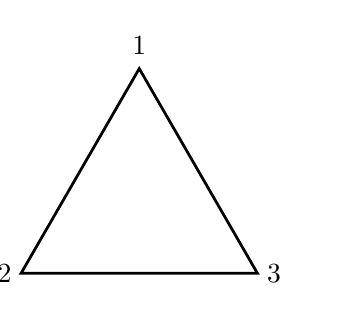
\begin{tikzpicture}
			\draw [black,line width=1pt] (0,0) -- (60:3) -- (3,0) -- cycle;
			\coordinate[label=left:$2$]  (2) at (0,0);
			\coordinate[label=right:$3$] (3) at (3,0);
			\coordinate[label=above:$1$] (1) at (1.5,2.65);
		\end{tikzpicture}
	\end{center}
	Using Cayley's theorem we can describe six symmetries using bijections, the identity symmetry;
	\begin{center}
		$id=\left(
		\begin{array}{c c c}
		1 & 2 & 3\\
		1 & 2 & 3
		\end{array}
		\right)$
	\end{center}
	Two rotational symmetries;
	\begin{center}
		$\left(
		\begin{array}{c c c}
		1 & 2 & 3\\
		2 & 3 & 1
		\end{array}
		\right),$
		$\left(
		\begin{array}{c c c}
		1 & 2 & 3\\
		3 & 1 & 2
		\end{array}
		\right)$
	\end{center}
	and three reflection symmetries;
	\begin{center}
		$\left(
		\begin{array}{c c c}
		1 & 2 & 3\\
		1 & 3 & 2
		\end{array}
		\right),$
		$\left(
		\begin{array}{c c c}
		1 & 2 & 3\\
		3 & 2 & 1
		\end{array}
		\right),$
		$\left(
		\begin{array}{c c c}
		1 & 2 & 3\\
		2 & 1 & 3
		\end{array}
		\right)$.
	\end{center}
	These describe it well enough to represent the entire shape, however there are some partial symmetries also. Just like with a full symmetry, we wish to shift the shape in such a way it appears the same, partial symmetries wish to shift "sub-shapes", like an edge or a vertex in this case, so that it appears the same. For the equilateral triangle, we have 3 edges and 3 vertices that can all be used for partial symmetries, and these are described using the following partial bijections;
	\begin{center}
		$\left(
		\begin{array}{c c}
		1 & 2 \\
		1 & 2 
		\end{array}
		\right),$
		$\left(
		\begin{array}{c c}
		1 & 2 \\
		2 & 3 
		\end{array}
		\right),$
		$\left(
		\begin{array}{c c}
		1 & 2\\
		1 & 3
		\end{array}
		\right),$
		$\left(
		\begin{array}{c c}
		1 & 3 \\
		1 & 3 
		\end{array}
		\right),$
		$\left(
		\begin{array}{c c}
		1 & 3\\
		1 & 2
		\end{array}
		\right),$
		$\left(
		\begin{array}{c c}
		1 & 3\\
		2 & 3
		\end{array}
		\right),$
		$\left(
		\begin{array}{c c}
		2 & 3 \\
		2 & 3 
		\end{array}
		\right),$
		$\left(
		\begin{array}{c c}
		2 & 3\\
		1 & 2
		\end{array}
		\right),$
		$\left(
		\begin{array}{c c}
		2 & 3\\
		1 & 3
		\end{array}
		\right)$.
	\end{center}
	We also have the mapping of the three vertices to each other vertex, described by the following partial bijections;
	\begin{center}
		$\left(
		\begin{array}{c}
		1 \\
		1
		\end{array}
		\right),$
		$\left(
		\begin{array}{c}
		1 \\
		2
		\end{array}
		\right)$,
		$\left(
		\begin{array}{c}
		1 \\
		3
		\end{array}
		\right)$,
		$\left(
		\begin{array}{c}
		2 \\
		1
		\end{array}
		\right)$,
		$\left(
		\begin{array}{c}
		2 \\
		2
		\end{array}
		\right)$,
		$\left(
		\begin{array}{c}
		2 \\
		3
		\end{array}
		\right)$,
		$\left(
		\begin{array}{c}
		3 \\
		1
		\end{array}
		\right)$,
		$\left(
		\begin{array}{c}
		3 \\
		2
		\end{array}
		\right)$,
		$\left(
		\begin{array}{c}
		3 \\
		3
		\end{array}
		\right)$.
	\end{center}
	When one compares this to $I_3$ from Example \ref{ex4.2} we can clearly see that the bijections are a subset of $I_3$, and so here we see the Wagner-Preston representation theorem in action, as all the partial symmetries of the equilateral triangle are embedded into $I_3$ using these partial bijections.\\
	Another thing of note is that clearly 
	$\left(
		\begin{array}{c c}
		1 & 2 \\
		3 & 2 
		\end{array}
		\right)$
	would also describe the partial symmetry of the sides $12$ and $23$, however only one bijection is required to describe the symmetry and as such it is embedded into $I_3$.
\end{ex}
\noindent In this case, the partial symmetries only involve sides and vertices of the main shape, and so they do not add too much extra information, however it is useful to describe these as it demonstrates what a partial symmetry actually is and how it is represented with a real example. With other objects that are not so simple, regular group mappings are not good enough to describe the complexity found and a lot of information would be lost, and here partial symmetries are much more numerous and more important.\\
\\There is a much more complex and interesting example which can directly demonstrate the power of inverse semigroups in \textbf{Sierpinski's triangle}.
\begin{ex}
Sierpinski's triangle is a fractal composed of equilateral triangles with the center quarter removed, as seen below;
	\begin{center}
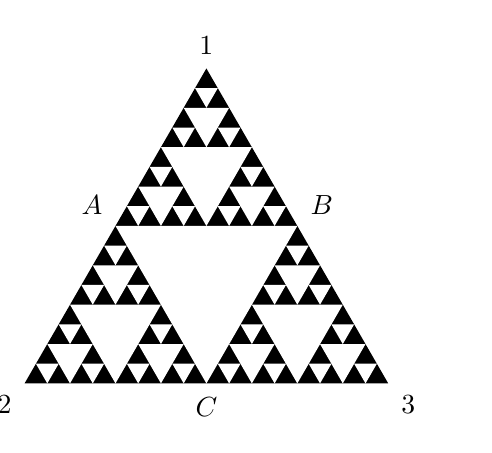
\begin{tikzpicture}[
main tri/.style={isosceles triangle,fill,isosceles triangle apex angle=60,
                 rotate=90,inner sep=0,outer sep=0},
filler tri/.style={isosceles triangle,fill=white,rotate=-90,isosceles triangle apex angle=60,
                 inner sep=0,outer sep=0}]
\node[minimum height=4cm,main tri,label={[label distance=0.5mm]0:$1$},label={[label distance=0.5mm]120:$2$},label={[label distance=0.5mm]240:$3$}] (a) {};
%==================
\node[minimum height=2cm,filler tri,label={[label distance=0.5mm]0:$C$},label={[label distance=0.5mm]120:$B$},label={[label distance=0.5mm]240:$A$}] (b) at (a.center){};
%==================
\node[minimum height=1cm,filler tri,anchor=right corner] (c1) at (b.left side){};
\node[minimum height=1cm,filler tri,anchor=left corner] (c2) at (b.right side){};
\node[minimum height=1cm,filler tri,anchor=apex] (c3) at (b.west){};
% ===================
\foreach \x in {1,2,3}{
\node[minimum height=0.5cm,filler tri,anchor=right corner] (d1\x) at (c\x.left side){};
\node[minimum height=0.5cm,filler tri,anchor=left corner] (d2\x) at (c\x.right side){};
\node[minimum height=0.5cm,filler tri,anchor=apex] (d3\x) at (c\x.west){};
}
% ===================
\foreach \x in {1,2,3}{
    \foreach \y in {1,2,3}{
    \node[minimum height=0.25cm,filler tri,anchor=right corner] (e1\x\y) at (d\x\y.left side){};
    \node[minimum height=0.25cm,filler tri,anchor=left corner] (e2\x\y) at (d\x\y.right side){};
    \node[minimum height=0.25cm,filler tri,anchor=apex] (e3\x\y) at (d\x\y.west){};
    }
}
\end{tikzpicture}
	\end{center}
Now consider the partial symmetries on this triangle. Clearly this is a much more complex shape than a plain equilateral triangle, however if one solely considers groups and Cayley's Theorem, then in fact this would be indistinguishable from the equilateral triangle found in Example \ref{ex.tri}. This is one of the easiest ways to demonstrate the significance of inverse semigroups and the Wagner-Preston representation theorem, as if we consider the partial bijections, we get much more information. For example, some of the partial bijections we have in this would be 
\begin{center}
	$\left(
		\begin{array}{c c c}
		1 & 2 & 3\\
		A & 2 & C
		\end{array}
		\right)$,
	$\left(
		\begin{array}{c c}
		1 & 2 \\
		C & B 
		\end{array}
		\right)$,
	$\left(
		\begin{array}{c c c}
		A & 2 & C\\
		B & C & 3
		\end{array}
		\right)$
\end{center}
The first of these describes the symmetry between the main triangle, and the second level triangle on the bottom left. From looking at them, it is clear that they are functionally identical, and this partial bijection captures this fact, whereas a (non-partial) bijection would not be able to describe this comparison at all, and the complexity would be lost.\\
The second of these partial bijections shows how the edge 12 on the main triangle is a partial symmetry to the edge CB on the smaller right triangle. Again this could not be captured by group symmetries and shows just how necessary partial bijections are even on this first example.\\
The third of these simply describes how two of the smaller triangles are partially symmetrical to each other, which is very apparent from looking at it but thanks to partial bijections can be described mathematically.\\
\end{ex}
\noindent This is one of the best examples as it can be so easily compared to the equilateral triangle to demonstrate the use and effectiveness of partial bijections. One thing worth noting is that in the case of the Sierpinski Triangle, this can be repeated ad infinitum, due to the fractal nature of the shape. What this means is that if one "zooms in" on any one triangle, the shape will appear completely identical to the starting shape, and this means that there is a partial bijection that can map any one of these triangles, edges or vertices no matter how small, onto the full triangle 123.
\subsection{Bicyclic Semigroup}
Our next example is the \textbf{bicyclic semigroup}. This is a semigroup $B = \mathbb{N}^0 \times \mathbb{N}^0$, where the operation $\cdot$ is defined such that
	\begin{center}
		$(a,b)\cdot(c,d) = (a - b + max\{b,c\},d - c + max\{b,c\}$
	\end{center}
for $(a,b), (c,d) \in B$. Let us show that this is a semigroup, regular and an inverse semigroup.
\begin{ex}
	We wish to show this operation is associative, so consider $(a,b),(c,d),(g,h) \in B$, then we have
	\begin{align*}
		&(a,b)\cdot ((c,d)\cdot(g,h)) = (a,b) \cdot (c-d+max\{d,g\},h-g+max\{d,g\})\\
		=&(a-b+max\{b,c-d+max\{d,g\}\},h-g-c+d+max\{b,c-d+max\{d,g\}\})
	\end{align*}
	and we also have
	\begin{align*}
		&((a,b)\cdot(c,d))\cdot(g,h) = (a-b + max\{b,c\},d-c + max\{b,c\})\cdot (g,h)\\
		=&(a-b+c-d + max\{d-c+max\{b,c\},g\},h-g + max\{d-c + max\{b,c\},g\}).
	\end{align*}
Now for this to be associative, we want to show that
	\begin{align*}
		&a-b+max\{b,c-d+max\{d,g\}\} = a-b+c-d + max\{d-c+max\{b,c\},g\} \qquad and\\[3mm]
		&h-g-c+d+max\{b,c-d+max\{d,g\}\} = h-g + max\{d-c + max\{b,c\},g\}
	\end{align*}
Cancelling the like terms $a-b$ on the first and $h-g$ on the second, we see that these become exactly the same equation, namely
	\begin{center}
		$max\{b,c-d+max\{d,g\}\} = c-d + max\{d-c+max\{b,c\},g\}$
	\end{center}
and so we need only work with this. the maximum function is linear, and as such we can take the $c-d$ inside and get
	\begin{center}
		$max\{b,max\{c,c-d+g\}\} = max\{max\{b,c\},c-d+g\}$.
	\end{center}
So if we can show that this is true, then it is associative. Let us consider the left hand side of the equation, then we have
	\begin{align*}
		max\{b,max\{c,c-d+g\}\} &= max\{b,c,c-d+g\}\\
						&= max\{max\{b,c\},c-d+g\}
	\end{align*}
which is the right hand side of what we wanted, hence $\cdot$ is associative and $(B,\cdot)$ is a semigroup.
\end{ex}
Next we wish to show it is a regular semigroup.
\begin{ex}
Consider some $(a,b)\in B$. Then clearly we can see that
	\begin{align*}
		(a,b)(b,a)(a,b) &= (a-b + max\{b,b\}, a-b + max\{b,b\})(a,b)\\
				&= (a-b-a+b + max\{a-b+max\{b,b\},a\}, b-a+max\{a-b+max\{b,b\},a\})\\
				&=(max\{a,a\},b-a+max\{a,a\})\\
				&=(a,b)
	\end{align*}
Hence $B$ is a regular semigroup.
\end{ex}
Next we shall show that $B$ is an inverse semigroup.
\begin{ex}
	First we wish to establish what idempotents look like in $B$. Consider $(e,f)$, then we can see that
	\begin{center}
		(e,f)(e,f)=(e-f+max\{f,e\}, f-e+max\{f,e\}).
	\end{center}
	Clearly if f=e then we get
	\begin{align*}
		(e,e)(e,e) &= (e-e+max\{e,e\},e-e+max\{e,e\})\\
			&= (e,e)
	\end{align*}
	And so all idempotents in $B$ take the form $(e,e)$.
	\\Using Proposition \ref{prop3.4}, we wish to show that for any two idempotents $(e,e),(f,f) \in B$, $(e,e)(f,f)=(f,f)(e,e)$. Consider the left hand side, then we have
	\begin{align*}
		(e,e)(f,f)&=(e-e+max\{e,f\},f-f+max\{e,f\})\\
			&= (max\{e,f\},max\{e,f\})\\
			&=(max\{f,e\},max\{f,e\})\\
			&=(f-f+max\{f,e\},e-e+max\{f,e\})\\
			&=(f,f)(e,e)
	\end{align*}
	Hence $B$ is a regular semigroup with commuting idempotents and by Proposition $\ref{prop3.4}$, $B$ is an inverse semigroup.
\end{ex}
\noindent We can clearly see that $B$ is an inverse monoid, as for any $(a,b) \in B$ we have the element $(0,0)$ as an identity, since
	\begin{align*}
		(a,b)(0,0) &= (b-a+max\{b,0\},0-0+max\{b,0\})\\
			&= (a,b)
	\end{align*}
with the same holding for $(0,0)(a,b)$.\\
\\This is one of the simpler examples of inverse semigroups, as the proofs for this allow you to work with natural numbers, however this is another nice example for demonstrating the more algebraic related side of semigroups. Whilst the example for Sierpinski's triangle is algebraically represented, it is to do with describing a geometric shape. In the case of the bicyclic semigroup however, it is an algebraic structure that can just as easily be described using the properties of inverse semigroups.
\section{Conclusion}
This project just scratches the surface of inverse semigroups, discussing the basic foundations and presenting some important theorems and examples, however there is a wide range of research still being carried out in this area. The applications to computer science in the ways discussed in the introduction keep this field relevant and thriving, as well as ensuring it stays relevant to a wide variety of fields in Mathematics. The basics of inverse semigroups presented in this project, from the properties to the Wagner-Preston Representation theorem, further concepts such as right and left ideals, Green relations, fuzzy semigroup and the free symmetric monoid can be researched, and the context provided here should give a strong foundation for these to build upon.\\
The aim of this project was to introduce the concepts of semigroups and inverse semigroups, providing some key results such as the Wagner-Preston Representation theorem and also discuss the partial order and natural partial order, some important and also intuitive concepts in inverse semigroups. These should all be taken as a basis, and the examples shown in this project are merely a small subset of the real scope of inverse semigroups, however through this project the foundations of knowledge should be in place to be able to progress onto further reading materials and gain a more in-depth and detailed insight to this subject matter.
\begin{thebibliography}{99}
\bibitem{1}C. Hollings, Some First Tantalizing Steps into Semigroup Theory, Math. Mag. 80, no. 5, 331-344
\bibitem{2}C. Hollings, The Early Development of the Algebraic Theory of Semigroups, Arch. Hist. Exact Sci. (2009) 63: 497. https://doi.org/10.1007/s00407-009-0044-3
\bibitem{3}J.M. Howie, Fundamentals of Semigroup Theory, Oxford University Press, 1995 
\bibitem{4}M.V. Lawson, Primer on Inverse Semigroups, Department of Mathematics, Heriot-Watt University
\bibitem{5}M.V. Lawson, Inverse Semigroups, The Theory of Partial Symmetries, World Scientific Publishing, 1998
\bibitem{6} J. A. de Séguier, Théorie des Groupes Finis: Élements de la Théorie des Groupes Abstraits, Paris, Gauthier-Villars, 1904. https://archive.org/details/thoriedesgroup00sguoft/page/8
\bibitem{7}A.H. Clifford, Arithmetic and ideal theory of abstract multiplication, Bull. Amer. Math. Soc., Volume 40, Number 4 (1934), 326-330. https://projecteuclid.org/euclid.bams/1183497371
\bibitem{8}J.D. Lawson, . "The earliest semigroup paper?." Semigroup forum 52.1 (1996): 55-60. <http://eudml.org/doc/135433>.
\end{thebibliography}
\end{document}

	$\left(
		\begin{array}{c c c}
		1 & 2 & 3\\
		2 & 1 & \times			% code for partial mappings%
		\end{array}
		\right)$
